
\section{Scale-up Server Scalability}
\label{sec:scale}

\subsection{Test-bed and Benchmark}

%$$$$$$$$$$$$$$$$$$$$$$$$$$$$$$$$$$$$$$$$$$$$$$$$$$$$$$$$$$$$$$$$$$$$$$$$$$$$$$$$
%$$$$$$$$$$$$$$$$$$$$$$$$$$$$$$$$$$$$$$$$$$$$$$$$$$$$$$$$$$$$$$$$$$$$$$$$$$$$$$$$
% Apache Spark에 대한 설명
%$$$$$$$$$$$$$$$$$$$$$$$$$$$$$$$$$$$$$$$$$$$$$$$$$$$$$$$$$$$$$$$$$$$$$$$$$$$$$$$$
\ifkor
\noindent
\textbf{Apache Spark. }
Apache Spark is a framework for large scale distributed computation.
Resilient Distributed Datasets(RDD) is a collection of partitions of records, 
and the RDD is managed as Least Recently Used(LRU), so when there is not enough
memory, Spark evicts the least recently used a partition from RDD.

%\begin{figure}[h]
%    \centering
%    \begin{subfigure}[b]{0.22\textwidth}
%        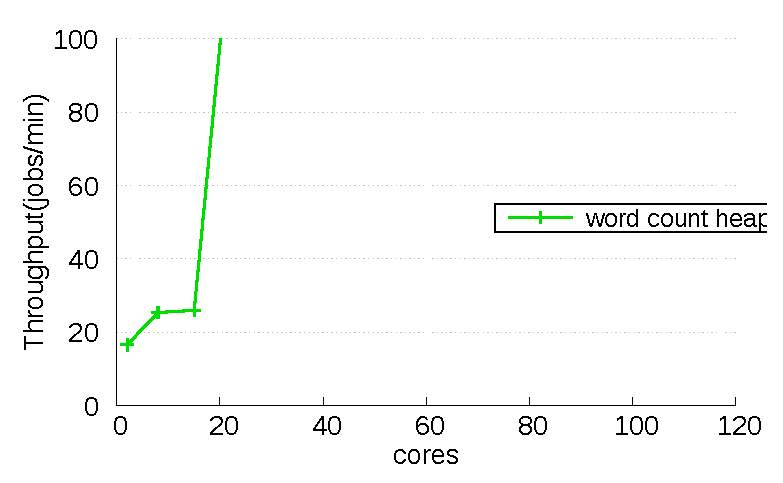
\includegraphics[width=1.5in]{graph/wc_max.eps}
%        \caption{Word Count}
%    \end{subfigure}%
%    \begin{subfigure}[b]{0.22\textwidth}
%        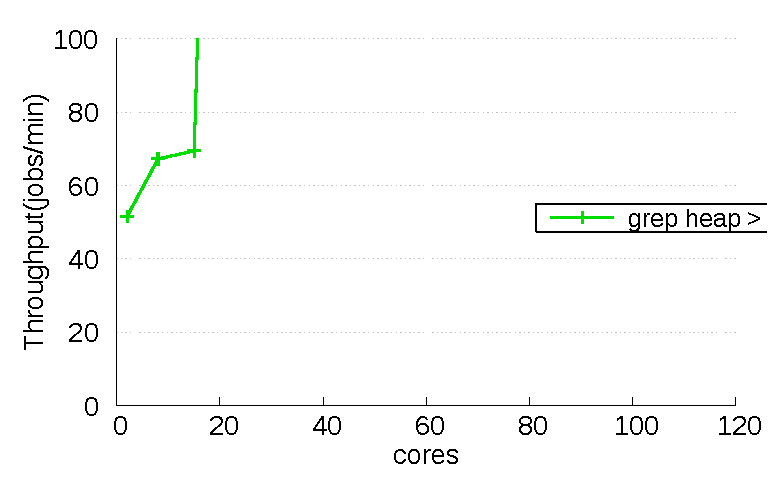
\includegraphics[width=1.5in]{graph/grep_max.eps}
%        \caption{Grep}
%    \end{subfigure}
%    \caption{CPU utilization on 120 core.}
%    \label{fig:utilization}
%\end{figure}

%Figure shows a substantial performance scalability of Spark when dataset can
% fit in memory(heap size > data size).
%However, large scale data(head size < data size) does not scale on scale-up
%server due to the GC and the memory latency.
\else
\fi

%$$$$$$$$$$$$$$$$$$$$$$$$$$$$$$$$$$$$$$$$$$$$$$$$$$$$$$$$$$$$$$$$$$$$$$$$$$$$$$$$
%$$$$$$$$$$$$$$$$$$$$$$$$$$$$$$$$$$$$$$$$$$$$$$$$$$$$$$$$$$$$$$$$$$$$$$$$$$$$$$$$
% 테스트 베드 설명
%$$$$$$$$$$$$$$$$$$$$$$$$$$$$$$$$$$$$$$$$$$$$$$$$$$$$$$$$$$$$$$$$$$$$$$$$$$$$$$$$
\ifkor
\noindent
\textbf{Test-bed. }
We used a machine to evaluate on real hardware: an 120-core (8 sockets × 15
cores) Intel Xeon E7-8870.
Hyper-Threading was disabled.


\begin{figure}[h]
  \begin{center}
     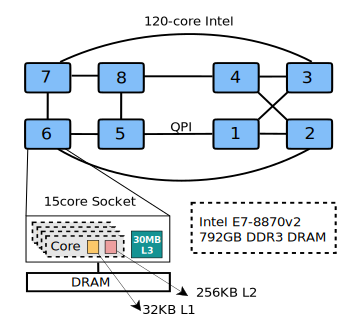
\includegraphics[width=0.3\textwidth]{fig/xeon}
  \end{center}
  \caption{Test-bed Intel Xeon architecture.}
  \label{fig:basic}
\end{figure}
\else

\fi

%$$$$$$$$$$$$$$$$$$$$$$$$$$$$$$$$$$$$$$$$$$$$$$$$$$$$$$$$$$$$$$$$$$$$$$$$$$$$$$$$
%$$$$$$$$$$$$$$$$$$$$$$$$$$$$$$$$$$$$$$$$$$$$$$$$$$$$$$$$$$$$$$$$$$$$$$$$$$$$$$$$
%Benchamrk에 대한 설명
%$$$$$$$$$$$$$$$$$$$$$$$$$$$$$$$$$$$$$$$$$$$$$$$$$$$$$$$$$$$$$$$$$$$$$$$$$$$$$$$$
\ifkor
\noindent
\textbf{Benchmark.} We used the BigDataBench.

\begin{table}[h!]
  \centering
  \small
  \begin{tabular}{l c c c c} \toprule
    Workload & Input data size & Heap size & Configuration & Data type\\
    \midrule
    Word Count & 10G & 4G & none & text \\ 
    Naive Basian & 10G & 4G & none & text\\
    Grep & 30G & 4G & \code{"the"} & text\\
    K-means & 4G & 4G & k=8 & graph\\
    \bottomrule
  \end{tabular}
  \begin{tabular}{l l l l l} \toprule
    JVM & Spark & Hadoop & OS & Distribution\\
    \midrule
    Openjdk 1.8.0\_91 & 1.3.1 & 1.2.1 & Linux 4.5-rc6 & Ubuntu 14.04\\ 
    \bottomrule
  \end{tabular}
  \caption{System information and configuration values.}
  \label{tab:memuse}
\end{table}

Table~\ref{tab:memuse} shows our configurations. we used four
workloads(Word Count, Naive Basian, Grep and K-means).
For the simplicity of experiment, we used input data size as the table~\ref{tab:memuse}.
Of course, large Spark heap size can eliminate the GC overhead, but commonly the
input data size is larger than the heap size in big data analytics area; we
used the smaller heap size than the input data size.

\else

\fi




\begin{figure*}[tb]
    \centering
    \begin{subfigure}[b]{0.25\textwidth}
        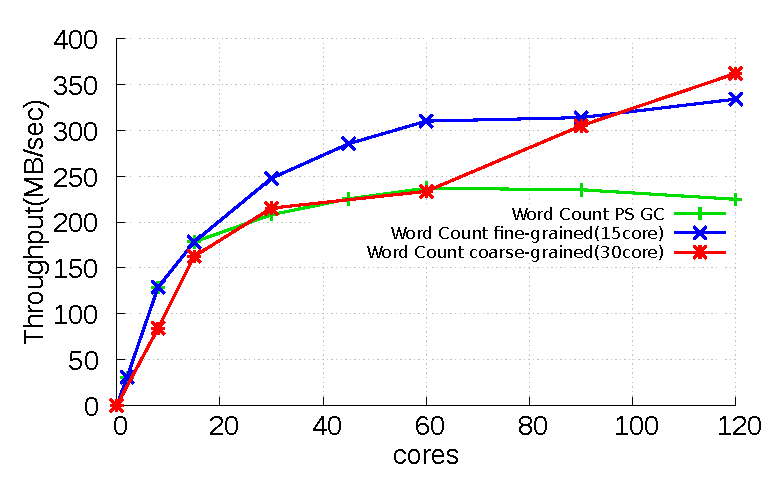
\includegraphics[width=1.8in]{graph/wc_docker.eps}
        \caption{Word Count}
    \end{subfigure}%
    \begin{subfigure}[b]{0.25\textwidth}
        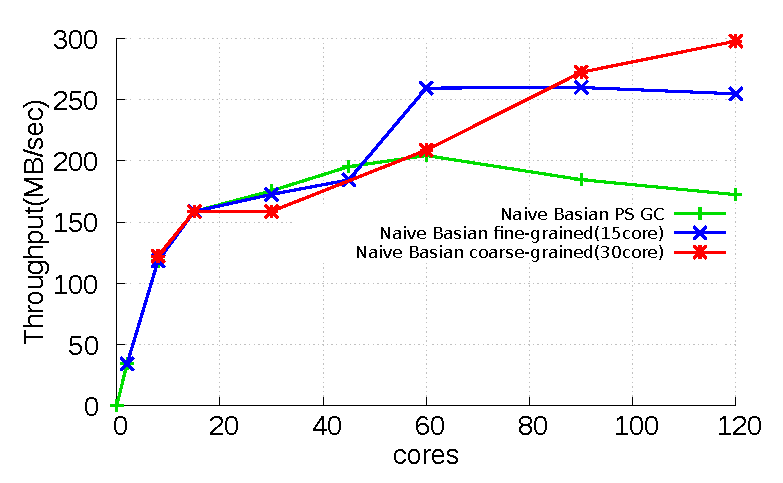
\includegraphics[width=1.8in]{graph/nb_docker.eps}
        \caption{Naive Basian}
    \end{subfigure}%
    \begin{subfigure}[b]{0.25\textwidth}
        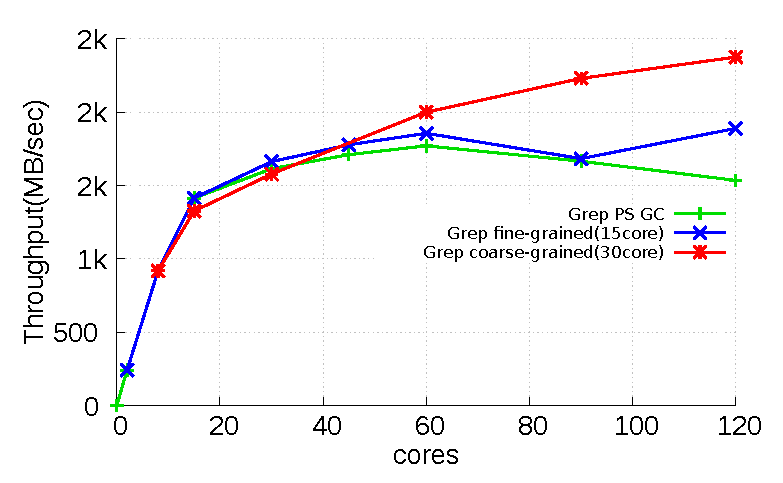
\includegraphics[width=1.8in]{graph/grep_docker.eps}
        \caption{Grep}
    \end{subfigure}%
    \begin{subfigure}[b]{0.25\textwidth}
        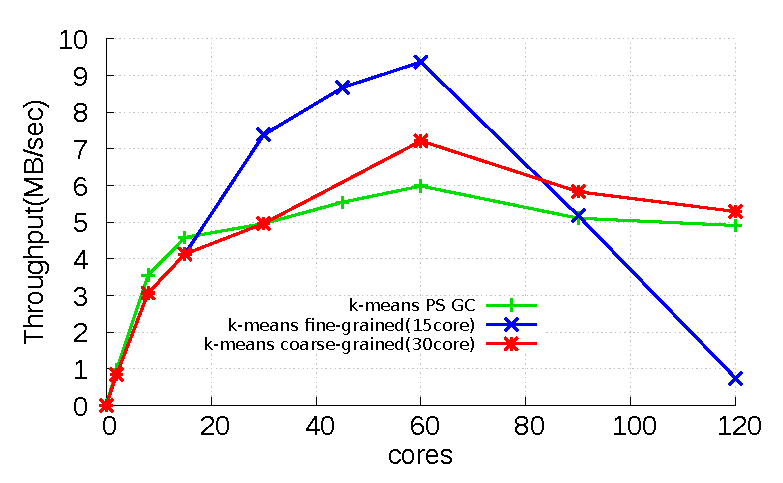
\includegraphics[width=1.8in]{graph/kmeans_docker.eps}
        \caption{K-means}
    \end{subfigure}%
    \caption{Performance scalability using docker container.}
    \label{fig:docker}
\end{figure*}


\begin{figure*}[tb]
    \centering
    \begin{subfigure}[b]{0.25\textwidth}
        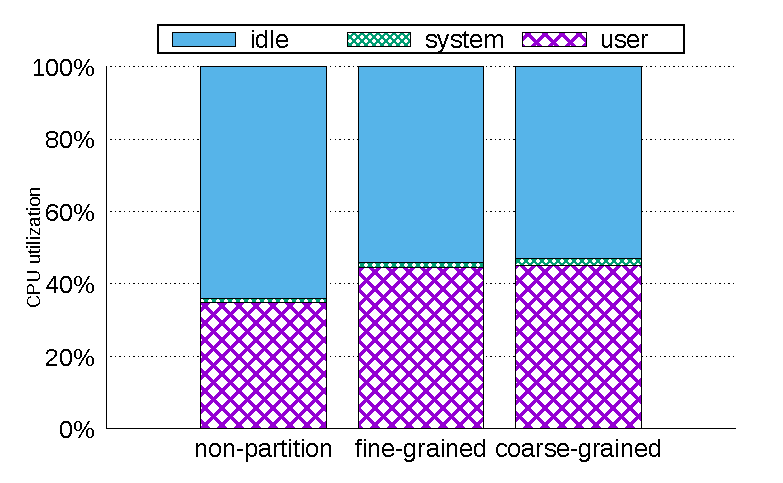
\includegraphics[width=1.8in]{graph/wc_cpuutils_docker.eps}
        \caption{Word Count}
    \end{subfigure}%
    \begin{subfigure}[b]{0.25\textwidth}
        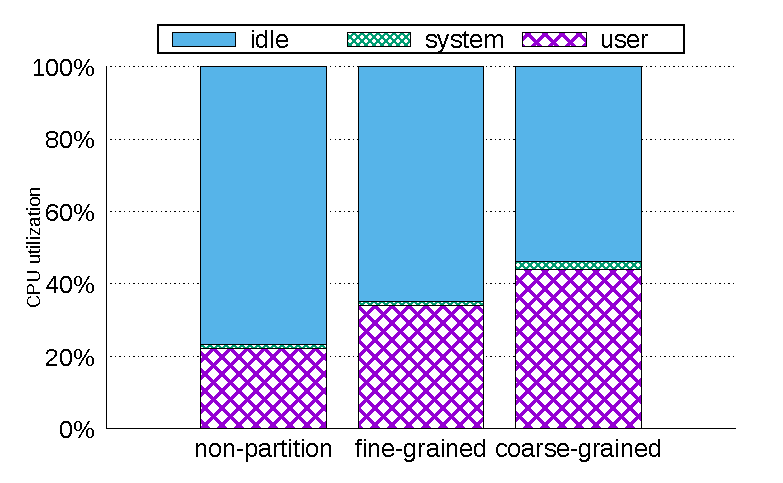
\includegraphics[width=1.8in]{graph/nb_cpuutils_docker.eps}
        \caption{Naive Basian}
    \end{subfigure}%
    \begin{subfigure}[b]{0.25\textwidth}
        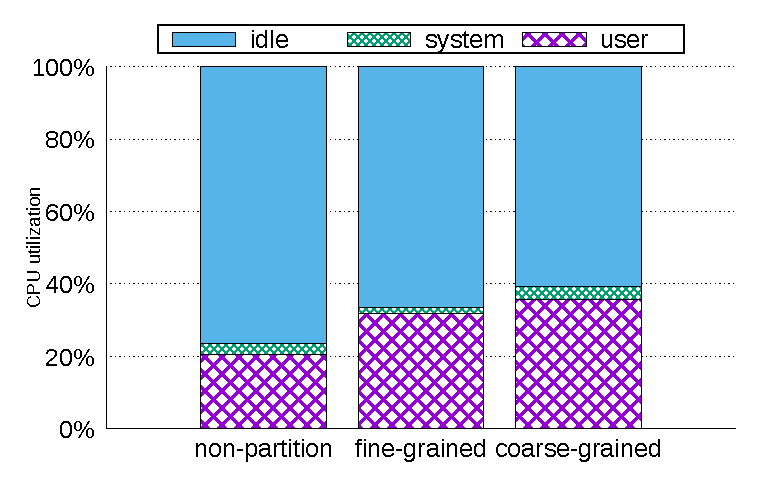
\includegraphics[width=1.8in]{graph/grep_cpuutils_docker.eps}
        \caption{Grep}
    \end{subfigure}%
    \begin{subfigure}[b]{0.25\textwidth}
        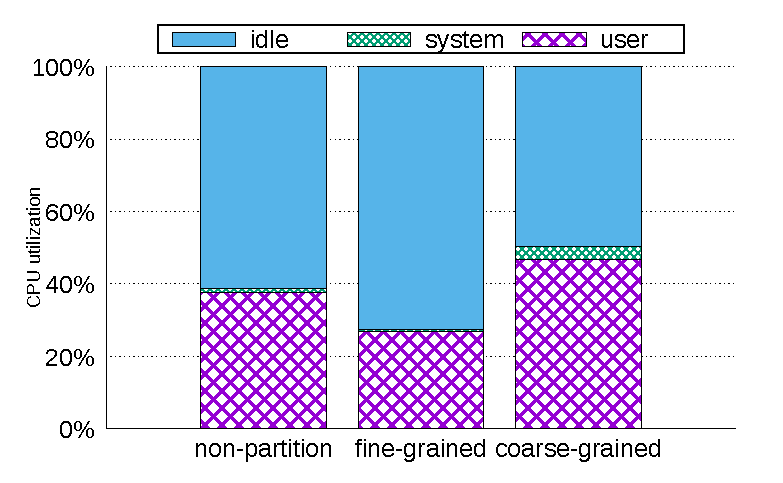
\includegraphics[width=1.8in]{graph/kmeans_cpuutils_docker.eps}
        \caption{K-means}
    \end{subfigure}%
        \centering
    \caption{CPU utilization on 120 core.}
    \label{fig:utilization2}
\end{figure*}



\subsection{Spark Scalability Problem}
%$$$$$$$$$$$$$$$$$$$$$$$$$$$$$$$$$$$$$$$$$$$$$$$$$$$$$$$$$$$$$$$$$$$$$$$$$$$$$$$$
%$$$$$$$$$$$$$$$$$$$$$$$$$$$$$$$$$$$$$$$$$$$$$$$$$$$$$$$$$$$$$$$$$$$$$$$$$$$$$$$$
%Scalability 결과에 대한 대략 적인 설명
%$$$$$$$$$$$$$$$$$$$$$$$$$$$$$$$$$$$$$$$$$$$$$$$$$$$$$$$$$$$$$$$$$$$$$$$$$$$$$$$$
Figure~\ref{fig:scalability} shows the Spark scalability of four workloads with
two state of the art garbage collections, G1 and Parallel Scavenge(PS).
Up to 60 core, the four workloads scale lineally and then GC pause becomes bottlenecks.
The Word Count workload flattens out after 60 core, and other benchmarks slightly go
down because not only the GC overhead but also the remote memory access. 
To evaluate state of the art GC, we compared the G1 with PS GC.
The effect of changing to the GC is the PS outperforms G1 up to 2.0x on 120 core.
Although we used the state of the art scalable GC,
the Spark performance scalability still suffers from GC.
Furthermore, we could not see any significant differences when increasing the size
of Spark executors.

%$$$$$$$$$$$$$$$$$$$$$$$$$$$$$$$$$$$$$$$$$$$$$$$$$$$$$$$$$$$$$$$$$$$$$$$$$$$$$$$$
%$$$$$$$$$$$$$$$$$$$$$$$$$$$$$$$$$$$$$$$$$$$$$$$$$$$$$$$$$$$$$$$$$$$$$$$$$$$$$$$$
%CPU utilization에 대한 설명
%$$$$$$$$$$$$$$$$$$$$$$$$$$$$$$$$$$$$$$$$$$$$$$$$$$$$$$$$$$$$$$$$$$$$$$$$$$$$$$$$

Our goal is to maximize CPU utilization, so we profiled the CPU utilization
on the four workloads.
Figure ~\ref{fig:cpuutilization} shows the CPU utilizations.
Th y-axis is the percentage of time spent in kernel-space code(sys), user-space
code(user), and idle time(idle).
All benchmarks increase the idle time due to the GC pause.

%$$$$$$$$$$$$$$$$$$$$$$$$$$$$$$$$$$$$$$$$$$$$$$$$$$$$$$$$$$$$$$$$$$$$$$$$$$$$$$$$
%$$$$$$$$$$$$$$$$$$$$$$$$$$$$$$$$$$$$$$$$$$$$$$$$$$$$$$$$$$$$$$$$$$$$$$$$$$$$$$$$
% Linux kernel scalability (lock, cache cohearnci, scheduler)등등 OS 노이즈에 대한 설명
%$$$$$$$$$$$$$$$$$$$$$$$$$$$$$$$$$$$$$$$$$$$$$$$$$$$$$$$$$$$$$$$$$$$$$$$$$$$$$$$$
\ifkor
%NUMA의 영향 뿐만 아니라, 추가적으로 operating system의 scalability 저해 요소 때문에 
%파티션닝 방법은 필요하다.
%우리는 operation system에서 scalability의 영향을 주는 것을 확인하기 위해 가장먼저
%lock을 조사해보았다.
%첫째로 공유 데이터를 lock이 있다. 표 xxx 앞에서 실험한 spark의 wordcount에 대해서 .
%JVM 위에서 동작하는 thread간의 공유하는 single address space때문에 발생하는 공유 문제이다.
%다음으로 scheduler가 아직 
%마지막으로 cache cohearci traffic이 있다. 
\else

\fi

\subsection{Benefit of JVM Partitioning}
%\subsection{NUMA}

\begin{figure}[h]
  \begin{center}
     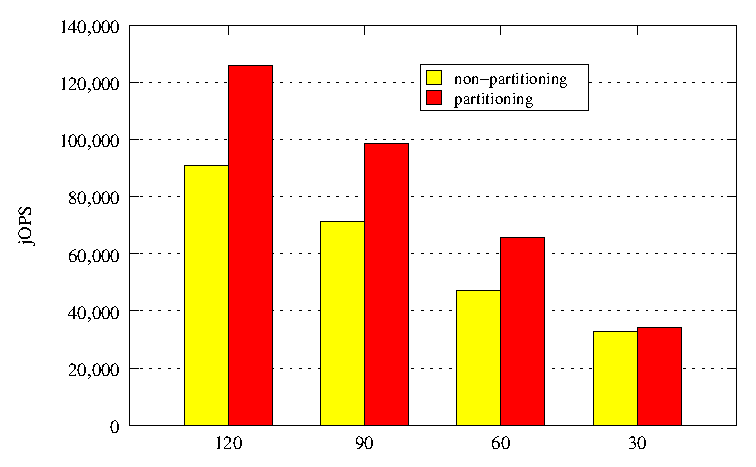
\includegraphics[width=0.4\textwidth]{graph/SPECjbb2013}
  \end{center}
  \caption{Effect on JVM partitioning.}
  \label{fig:SPECJBB}
\end{figure}

%$$$$$$$$$$$$$$$$$$$$$$$$$$$$$$$$$$$$$$$$$$$$$$$$$$$$$$$$$$$$$$$$$$$$$$$$$$$$$$$$
%$$$$$$$$$$$$$$$$$$$$$$$$$$$$$$$$$$$$$$$$$$$$$$$$$$$$$$$$$$$$$$$$$$$$$$$$$$$$$$$$
%NUMA 영향에 대한 대략 적인 설명
%$$$$$$$$$$$$$$$$$$$$$$$$$$$$$$$$$$$$$$$$$$$$$$$$$$$$$$$$$$$$$$$$$$$$$$$$$$$$$$$$

Spark and Hadoop frameworks use JAVA, and they need java virtual machine(JVM), so
understanding the JVM partitioning is important.
To preliminary evaluate the JVM partitioning effect, we conducted experiments
by using SPECjbb2013~\cite{Pogue2014SO}, which is a state of the art
benchmark for JVM performance.
We used two different experimental settings. 
First, we used per-socket JVM partitioning by using the NUMA control application(numactl).
Second, we set maximum JVM heap size, an available system
memory size, and all threads are scheduled by the OS to
migrate any core, and we enable automatic NUMA
balancing feature in the Linux kernel.

The results shows that partitioning approach outperforms non-partitioning approach
by 1.4x on 120 core(figure~\ref{fig:SPECJBB}).
Therefore, in manycore scale-up server, partitioning approach has many
advantages over non-partitioning approach in terms of performance scalability.

\subsection{Benefit of Container-based Partitioning}
\label{sec:eval}


%$$$$$$$$$$$$$$$$$$$$$$$$$$$$$$$$$$$$$$$$$$$$$$$$$$$$$$$$$$$$$$$$$$$$$$$$$$$$$$$$
%Paragraph 1: 실험 환경 설명
%$$$$$$$$$$$$$$$$$$$$$$$$$$$$$$$$$$$$$$$$$$$$$$$$$$$$$$$$$$$$$$$$$$$$$$$$$$$$$$$$
In this section we discuss the docker container-based partitioning on the
scale-up server described as section~\ref{sec:scale}.
We used ram file system for HDFS due to eliminating the HDFS bottleneck.


\begin{table}[h!]
  \centering
  \small
  \begin{tabular}{l r r} \toprule
    method & executor heap size & number of partitions\\
    \midrule
    non-partition & 4G & 1  \\ 
    coarse-grained(30 core) & 1G & 4\\
    fine-grained(15 core) & 512M & 8\\
    \bottomrule
  \end{tabular}
  \caption{Partitioning values.}
  \label{tab:memusepart}
\end{table}




%$$$$$$$$$$$$$$$$$$$$$$$$$$$$$$$$$$$$$$$$$$$$$$$$$$$$$$$$$$$$$$$$$$$$$$$$$$$$$$$$
%Paragraph 2: 비교 대상 설명
%$$$$$$$$$$$$$$$$$$$$$$$$$$$$$$$$$$$$$$$$$$$$$$$$$$$$$$$$$$$$$$$$$$$$$$$$$$$$$$$$
%기본으로 4G의 메모리를 heap 메모리 사이즈로 설정하였고, input 데이터는 10G 이상으로 설정하였다.
We used three different experiment settings.
First, we used the non-partitioning method as section~\ref{sec:scale}(heap size is 4G).
Second, we used a fine-grained partitioning(15 core) 
because it can maximize the NUMA locality.
%We allocated heap size by modifying heap size is that we divide 4G of number of
%partitioning.
%우리는 모든 파티션된 도커들의 executor에 대한 heap 메모리 사이즈는 non-partitioning에 method에서 사용한 힙사이즈(4)를 피티션 수로 나누어 사용하였다.
Table~\ref{tab:memusepart} shows our partitioning values.
The heap size of executor in the partitioned Docker is divided
by number of partitions.
Finally, we used the coarse-grained partitioning(30 core) 
since it can mitigate a straggler tasks problem~\cite{Ousterhout2015MSP}~\cite{Ren2015HDS}.

%$$$$$$$$$$$$$$$$$$$$$$$$$$$$$$$$$$$$$$$$$$$$$$$$$$$$$$$$$$$$$$$$$$$$$$$$$$$$$$$$
%Paragraph 2: WC, NB 결과 설명 
%$$$$$$$$$$$$$$$$$$$$$$$$$$$$$$$$$$$$$$$$$$$$$$$$$$$$$$$$$$$$$$$$$$$$$$$$$$$$$$$$
The results for Word Count are shown in Figure~\ref{fig:docker}(a).
Up to 60 core, the PS GC version of non-partitioning approach scales linearly and
then it flattens out.
However, up to 60 core, our fine-grained partitioning outperforms non-partitioning
since it can remove GC and NUMA latency overheads, and then a straggler tasks
problem become bottlenecks.
Our coarse-grained partitioning outperforms non-partitioning by 1.5x and
fine-grained partitioning by 1.1x on 120 core.
Furthermore, the non-partitioning approach has the highest idle time(64\%) since
GC becomes bottleneck(see figure~\ref{fig:utilization2}). 
The results(Figure~\ref{fig:docker}(b)) for Naive Bayesian is similar to Word Count
workload.
Our coarse-grained partitioning outperforms non-partitioning by 1.5x and fine-grained
by 1.2x on 120 core.


%$$$$$$$$$$$$$$$$$$$$$$$$$$$$$$$$$$$$$$$$$$$$$$$$$$$$$$$$$$$$$$$$$$$$$$$$$$$$$$$$
%Paragraph 3: Grep 결과 설명 
%$$$$$$$$$$$$$$$$$$$$$$$$$$$$$$$$$$$$$$$$$$$$$$$$$$$$$$$$$$$$$$$$$$$$$$$$$$$$$$$$
The results for Grep are shown in Figure~\ref{fig:docker}(c).
After to 60 core, the coarse-grained partitioning approach scales linearly, but
the others throughput go down after to 60 core because non-partitioning
version suffers from GC.
The fine-grained partitioning approach suffers from the straggler tasks problem.
Although the fine-grained partitioning approach eliminates the GC overhead and
the remote memory access, its CPU utilization(23\%) is low than coarse-grained partitioning(38\%).
Our coarse-grained partitioning outperforms non-partitioning by 1.5x and fine-grained
by 1.3x on 120 core.

%$$$$$$$$$$$$$$$$$$$$$$$$$$$$$$$$$$$$$$$$$$$$$$$$$$$$$$$$$$$$$$$$$$$$$$$$$$$$$$$$
% Paragraph 4: K-means 결과 설명 
%$$$$$$$$$$$$$$$$$$$$$$$$$$$$$$$$$$$$$$$$$$$$$$$$$$$$$$$$$$$$$$$$$$$$$$$$$$$$$$$$
The results for K-means are shown in Figure~\ref{fig:docker}(d),
The K-means workload suffers from GC~\cite{Ahsan2016SVS}; therefore,
fine-grained partitioning approach has substantial performance scalability up to 60 core.
However, then it collapses since it extremely suffers from the
straggler tasks problem that extends job completion times.
Our coarse-grained partitioning outperforms non-partitioning by 1.1x on 120 core.
Fine-grained partitioning approach has the lowest(72\%) idle time because the coarse-grained 
partitioning approach relatively less suffers from the straggler tasks problem.

